\documentclass[12pt]{article}
%\topmargin=-0.5in
%\textheight=9in
%\evensidemargin=0in
%\oddsidemargin=0in
%\setlength{\textwidth}{6.5in}

% Replace "Thesis Title", "Student name" etc. below with the correct values
% These values will then be automatically added wherever necessary in thesis-template.tex and defence-announcement.tex

\newcommand{\thesistitle}{Multilingual Digital Signage using Computer Vision and Bluetooth Beacons}
\newcommand{\studentname}{Suhas Dwarakanath}
\newcommand{\advisorname}{Dr. Brian Thoms}

% Custom commands for other often used strings (\pythonversion, \submissionyear etc.) can be added
% below using the following template
% \newcommand{\<commandname>}{<commandvalue>} 

\usepackage{amsmath,latexsym}
\usepackage{amsfonts}
\usepackage{amssymb}
\usepackage{amssymb}
\usepackage{graphicx}
%\usepackage{appendix}
%\usepackage{clrscode3e}
\usepackage{epstopdf}
\usepackage{subfigure}
%\usepackage{algorithm}
%\usepackage{algorithmic}
\usepackage{setspace}
\usepackage{color}
\usepackage{listings}
\usepackage{setspace}
\usepackage{algpseudocode}
\usepackage{algorithm}
\usepackage[all]{xy}
\usepackage{pdfpages}
\usepackage{titlesec}

% Ensures a new section is on its own page. Must be done before hyperref is loaded

%changed by Suhas

 \newcommand{\sectionbreak}{\clearpage}

% Clickable references
\usepackage[hidelinks]{hyperref}

% Ensures graphic is in view after clicking on a reference to see it
\usepackage[all]{hypcap} 


% \doublespacing
\renewcommand{\topfraction}{0.9}	% max fraction of floats at top
\renewcommand{\bottomfraction}{0.8}	% max fraction of floats at bottom

%   Parameters for TEXT pages (not float pages):
\setcounter{topnumber}{2}
\setcounter{bottomnumber}{2}
\setcounter{totalnumber}{4}      % 2 may work better
\setcounter{dbltopnumber}{2}    % for 2-column pages
\renewcommand{\dbltopfraction}{0.9}	% fit big float above 2-col. text
\renewcommand{\textfraction}{0.07}	% allow minimal text w. figs

%   Parameters for FLOAT pages (not text pages):
\renewcommand{\floatpagefraction}{0.7}	% require fuller float pages
    
% N.B.: floatpagefraction MUST be less than topfraction !!
\renewcommand{\dblfloatpagefraction}{0.7}	% require fuller float pages

\newenvironment{dig}{\\ [6pt]\noindent {\bf Digression}}{~$\Box$\\ [6pt]\indent}
\newenvironment{dig1}{\noindent {\bf Digression}}{~$\Box$\\ [6pt]\indent}
\newtheorem{alg}{\hspace{1.3in} Algorithm}
\newtheorem{thrm}{Theorem}
\newtheorem{lemm}[thrm]{Lemma}
\newtheorem{conj}[thrm]{Conjecture}
%\newtheorem{claim}[thrm]{Claim}
\newtheorem{prop}[thrm]{Proposition}
\newtheorem{defn}[thrm]{Definition}
\newtheorem{obs}[thrm]{Observation}

\hyphenation{Chris-to-dou-lak-is}
\def\proof{\bigbreak\noindent {\sl Proof.\/}\enspace}
\def\qedbox#1#2{\vbox{\hrule height.2pt
  \hbox{\vrule width.2pt height#2pt \kern#1pt \vrule width.2pt}
  \hrule height.2pt}}
\def\qed{\hfill \quad\qedbox46\newline\smallbreak}

\def\s#1{\mbox{\boldmath $#1$}}
\def\floor#1{\lfloor #1 \rfloor}
\def\bfloor#1{\big\lfloor #1 \big\rfloor}
\def\Bfloor#1{\Big\lfloor #1 \Big\rfloor}
\def\ceil#1{\lceil #1 \rceil}
\def\bceil#1{\big\lceil #1 \big\rceil}
\def\+{\!+\!}
\def\-{\!-\!}
\def\plmi{\!\pm\!}
\def\m{\!-\!}
\def\uu#1{\underline{#1}}
\def\o#1{\overline{#1}}
\def\itbf#1{\textit{\textbf{#1}}}
\def\match{\approx}
\def\cP{\mathcal{P}}
\def\G{\mathcal{G}}
\def\B{\mathcal{B}}
\def\O{\mathcal{O}}

\def\bproc{{\bf procedure\ }}
\def\bfunc{{\bf function\ }}
\def\bvar{{\bf var\ }}
\def\barray{{\bf array\ }}
\def\bof{{\bf of\ }}
\def\bfor{{\bf for\ }}
\def\bnull{{\bf null\ }}
\def\bto{{\bf to\ }}
\def\bdownto{{\bf downto\ }}
\def\bwhile{{\bf while\ }}
\def\brep{{\bf repeat\ }}
\def\buntil{{\bf until\ }}
\def\band{{\bf and\ }}
\def\bor{{\bf or\ }}
\def\bdo{{\bf do\ }}
\def\bif{{\bf if\ }}
\def\bthen{{\bf then\ }}
\def\belse{{\bf else\ }}
\def\belsif{{\bf elsif\ }}
\def\bnot{{\bf not\ }}
\def\bgoto{{\bf goto\ }}
\def\bcontinue{{\bf continue\ }}
\def\breturn{{\bf return\ }}
\def\bbreak{{\bf break\ }}
\def\boutput{{\bf output}}
\def\la{\leftarrow}
\def\ra{\rightarrow}
\def\llra{\Leftrightarrow}
\def\q{\quad}
\def\qq{\qquad}
\def\com#1{{\bf $\triangleright$}\hspace{6pt}{\sl #1}}
\def\rem#1{\hspace{24pt}{\sl #1}}
\def\pref(#1,#2){$#1$ is a prefix of $#2$}
\def\suff(#1,#2){$#1$ is a suffix of $#2$}
\def\FIND{\mbox{FIND}}
\def\reg(#1,#2){$#2$ is $#1$-regular}
\def\notreg(#1,#2){$#2$ is not $#1$-regular}
\def\top{\tt{top}}
\def\pop{\tt{pop}}
\def\push{\tt{push}}
\def\true{\tt{true}}
\def\false{\tt{false}}
\def\UPDATE\_F{\tt{UPDATE\_F}}
\def\LEAST{\tt{LEAST}}
\def\MERGE{\tt{MERGE}}
\def\mec{\tt{mec}}
\def\MEC{\tt{MEC}}
\def\CMEC{\tt{CMEC}}
\def\MELC{\tt{MELC}}
\def\CMELC{\tt{CMELC}}
\def\MELS{\tt{MELS}}
\def\CMELS{\tt{CMELS}}
\def\MCNT{\tt{MaxCount}}
\def\CLEN{\tt{CorLen}}

% \def\B{\tt{B}}
\def\Q'{\tt{Q'}}
\def\CP{\tt{CP}}
\def\MNC{\tt{MNC}}
\def\PR{\tt{PR}}
\def\PRS{\tt{PRS}}
\def\CPR{\tt{CPR}}
% \def\POS{\tt{POS}}
\def\LEN{\tt{LEN}}
\newcommand{\dd}{\mathinner{\ldotp\ldotp}}

\newif\ifShow
\Showfalse
% MATH -----------------------------------------------------------
\newcommand{\norm}[1]{\left\Vert#1\right\Vert}
\newcommand{\abs}[1]{\left\vert#1\right\vert}
\newcommand{\set}[1]{\left\{#1\right\}}
\newcommand{\Real}{\mathbb R}
\newcommand{\eps}{\varepsilon}
\newcommand{\To}{\longrightarrow}
\newcommand{\BX}{\mathbf{B}(X)}
\newcommand{\A}{\mathcal{A}}
% Algorithm ------------------------------------------------------

\algnewcommand{\LineComment}[1]{\State \(\triangleright\) \normalfont{\sl #1}}
\algtext*{EndWhile}% l
\algtext*{EndIf}% Remove "end if" text
\algtext*{EndFor}% Remove "end for" text
\algtext*{EndFor}% Remove "end for" text
\algtext*{EndProcedure}% Remove "end procedure" text

% manifold
\newcommand{\F}{{F}}
\newcommand{\scF}{\F}
\newcommand{\X}{{X}}
\newcommand{\Fhat}{\widehat\F}
\newcommand{\scN}{{\EuScript N}}
\newcommand{\scL}{{\EuScript L}}
\newcommand{\PP}{\mathbb P}
\newcommand{\R}{\mathbb R}
\newcommand{\C}{\mathbb C}
% \newcommand{\CP}{\C\PP}
\newcommand{\CH}{\C{\mathrm H}}
\newcommand{\Lie}{{\mathcal L}}
\newcommand{\cpn} {\CP^n}
\newcommand{\chn} {\CH^n}
\newcommand{\cptwo} {\CP^2}
\newcommand{\chtwo} {\CH^2}
\newcommand{\chone} {\CH^1}
%\newcommand{\mean}{{\mathcal m}}
\newcommand{\mean}{{\mathbf m}}
%\def\({\left (}
\def\({\left(}
%\def\){\right )}
\def\){\right)}
\def\<{\langle}
\def\>{\rangle}
\def\a {\alpha}
\def\b {\beta}
\def\l {\lambda}

% Pfaffian systems
\newcommand{\CC}{{\EuScript C}}
\newcommand{\I}{{\mathcal I}}
\newcommand{\J}{{\EuScript J}}
\newcommand{\K}{{\mathcal K}}
\newcommand{\Khat}{\widehat{\K}}
\newcommand{\M}{{\mathcal M}}
\newcommand{\V}{\mathcal V}
\newcommand{\calS}{\mathcal S}

% differential forms
\newcommand{\w}{\omega}
\newcommand{\kh}{\hat\kappa}
\newcommand{\diff}{{\operatorname{diff}}}
% \newcommand{\alg}{{\operatorname{alg}}}

%maps
\newcommand{\fhat}{\hat{f}}

%open sets
\newcommand{\setU}{\EuScript U}
\newcommand{\Uhat}{\widehat{\setU}}

% vectors
\newcommand{\e}{\mathbf e}
\newcommand{\ehat}{\hat{\e}}
\newcommand{\bv}{\mathbf v}
\newcommand{\bx}{\mathbf x}
\newcommand{\bg}{\mathbf g}
\newcommand{\by}{\mathbf y}
\newcommand{\bw}{\mathbf w}
\newcommand{\bxi}{\mathbf\xi}
\newcommand{\bn}{\mathbf n}
\newcommand{\bz}{\mathbf z}

% complex variables
\newcommand{\ri}{\mathrm i}
\newcommand{\realpart}{\operatorname{Re}}

% operators
\newcommand{\JJ}{{\mathrm J}} % complex structure
\newcommand{\RR}{{\sf R}} % curvature operator
\newcommand{\Ric}{{\sf Ric}} % Ricci tensor
\newcommand{\di}{\partial}
\newcommand{\dib}[1]{\di_{#1}}
\newcommand{\tvec}{\tfrac{\di}{\di t}}
\newcommand{\restr}{\negthickspace \mid}
\newcommand{\transpose}[1]{{}^t\hskip-2pt{#1}}
\newcommand{\nat}{\widetilde\nabla}
\newcommand{\RRt}{\widetilde R}
\newcommand{\mt}{\widetilde M}
\def\intprod{\mathbin{\raisebox{.4ex}{\hbox{\vrule height .5pt width
5pt depth 0pt %
         \vrule height 3pt width .5pt depth 0pt}}}}
\newcommand{\hook}{\intprod}
\def\&{\wedge}
% \def\s{\sigma}
\def\a{\alpha}
\def\b{\beta}
\def\n{\nabla}

\title{\thesistitle} 
\author{\studentname}
\date{\today}

\begin{document}

\begin{titlepage}
\pagenumbering{gobble}
\begin{center}
{\Large \bfseries \thesistitle \par}

\vspace{2 cm}
\baselineskip = 2\baselineskip
A Thesis Presented to \\
The Faculty of the Computer Science Department\\
California State University Channel Islands

\vspace{1 cm}

In (Partial) Fulfillment\\
of the Requirements for the Degree\\
Masters of Science in Computer Science\\

\vspace{1 cm }

\vfill

by \\
\studentname\\
Advisor: \advisorname\\
March 2019
\end{center}
\end{titlepage}
\baselineskip = \baselineskip
\newpage

\null
\vfill
\begin{flushleft}
\copyright\; 2019\\
\studentname\\
ALL RIGHTS RESERVED
\end{flushleft}
\newpage

\begin{center}
{\large \bfseries APPROVED FOR MS IN COMPUTER SCIENCE \par}

\vspace{1.5 cm}

\hrulefill\\
{\large \bfseries Advisor: \advisorname \hfill Date \par}

\vspace{1.5 cm}

\hrulefill\\
{\large \bfseries Name \hfill Date \par}

\vspace{1.5 cm}

\hrulefill\\
{\large \bfseries Name \hfill Date \par}

\vspace{3 cm}

{\large \bfseries APPROVED FOR THE UNIVERITY \par}

\vspace{1.5 cm}

\hrulefill\\
{\large \bfseries Name \hfill Date \par}
\end{center}
\newpage

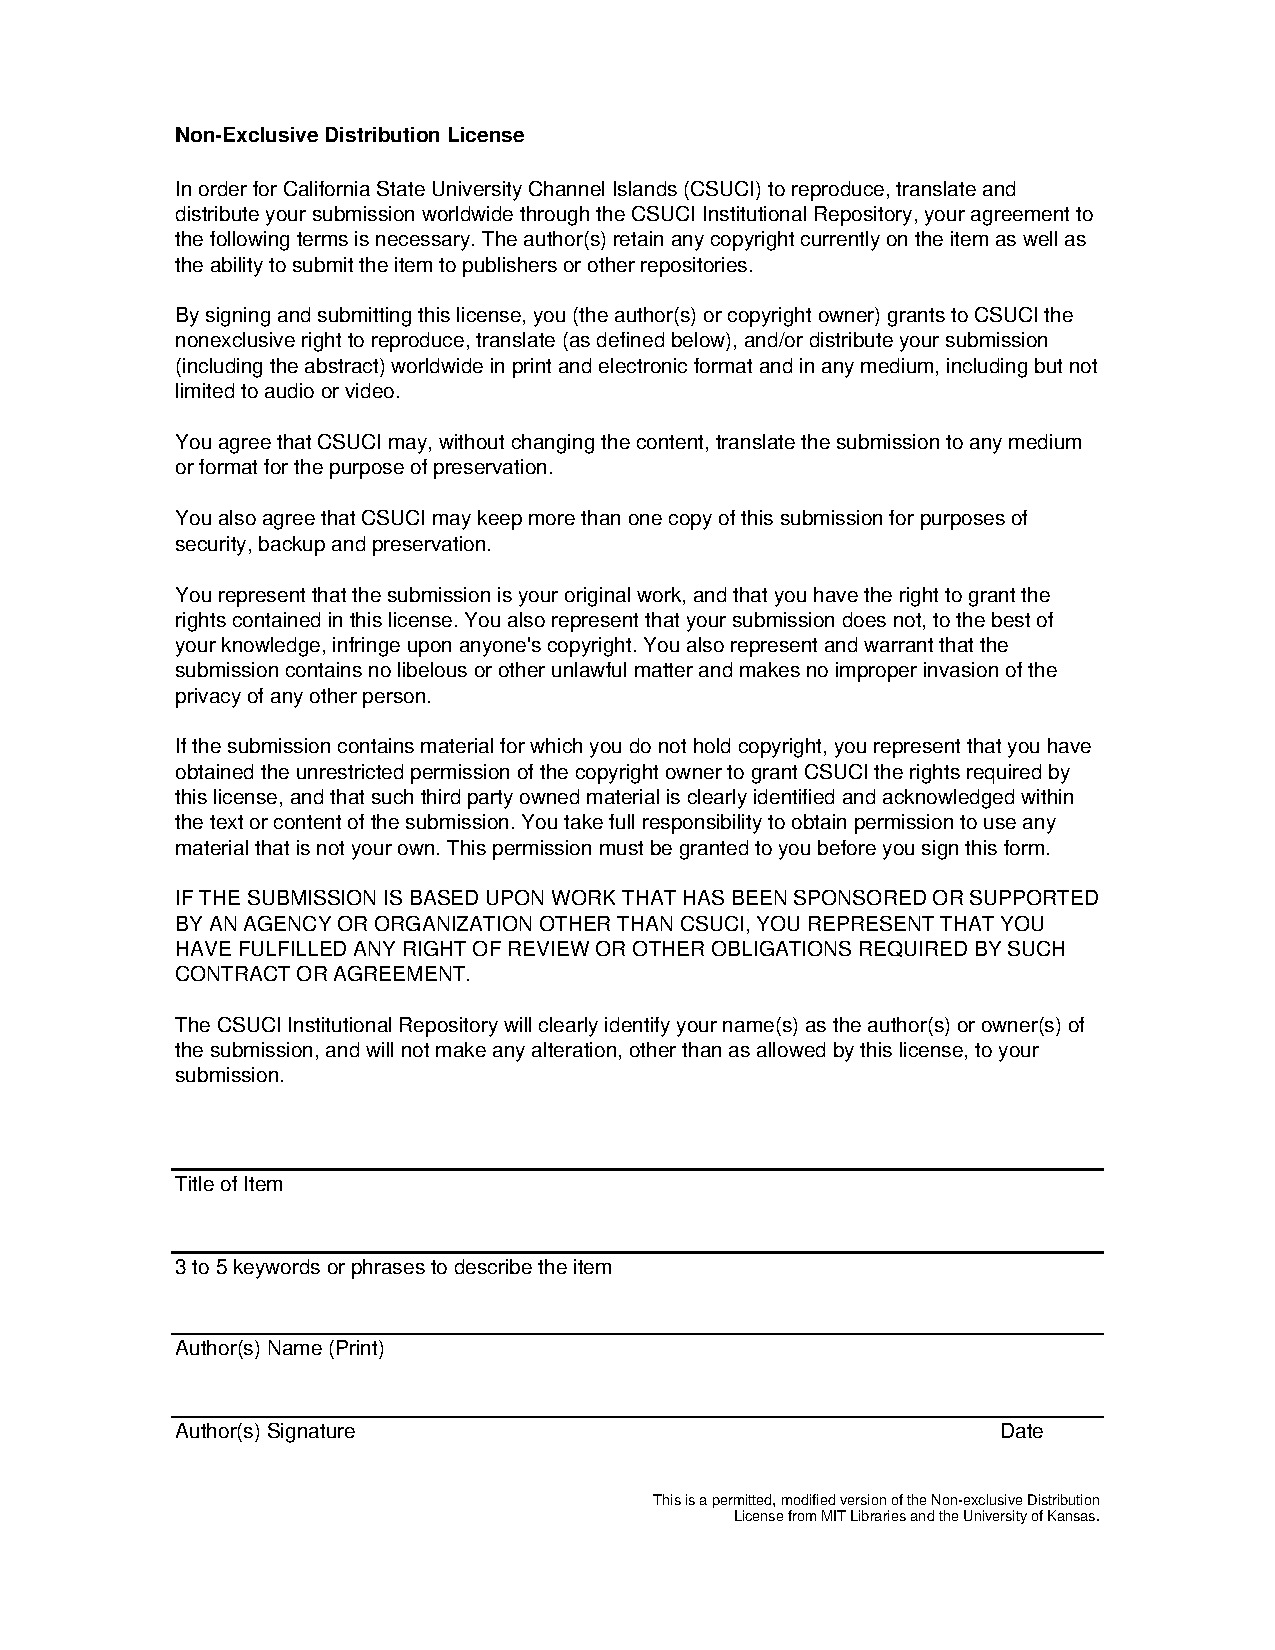
\includepdf{media/distribution-license.pdf}
\newpage


\maketitle

\begin{abstract}
Due to globalization and changing lifestyle, more and more people are visiting foreign countries for business and travel. Also lately, a lot of newly arriving refugee families to the U.S face legal consequences. One of the struggles they face is reading documentation they receive through mail; whether bills, court documents or financial assistance documents, they struggle to read and understand them. There are thousands of languages in the world and it is impractical to install signage and print documents in all the languages. In this research, by combining Computer Vision and Bluetooth beacons, multilingual digital information is displayed on the user's smartphone. Smartphone camera allows the user to take a picture of a document. It is then posted to the Google Cloud Vision API which returns the text of that document. It can then be translated to any language using Google Translate API. The system also displays the information of nearby signages (with bluetooth beacons) on the smartphone. This system was implemented in the university campus and the evaluation experiment was conducted by on international students. It was found that the system helps the users to understand their environment better in their native language.
\end{abstract}

\newpage
\pagenumbering{roman}

\tableofcontents

\newpage

\listoffigures

\newpage
\pagenumbering{arabic}

\section{Introduction}
\label{sect-intro}

With changing lifestyle and globalization, more people visit foreign countries. Every country is working towards becoming tourism oriented to increase their economy. Most of the visitors use their smartphone to access information. However, when visiting foreign countries, most people face difficulties in obtaining information due to difference in language, which makes it an inconvenience to stay in foreign countries for a longer time.  \\

Recently, a lot of refugee and migrant families from all over the world faced a lot of struggles at the U.S immigrations. A lot of these refugees faced problems with the documentation because they could not understand the content of the legal documents. It is natural for people to understand information better in their home language. Therefore, an effective method of providing and accessing information in multiple languages is required. \\

In this study, in order to solve such problems, a multilingual information service was developed using Computer Vision and Bluetooth beacons. The information can be accessed from the user's smartphone in most of the languages. We focus on the smartphone's camera to 'see' information in multiple languages. We also use bluetooth beacons to 'push' information to smartphones in proximity. The user can then access the information in multiple languages. By using this method, we expect people visiting foreign countries to access information naturally in the same way they would in their home countries. This paper evaluates various options like GPS, NFC and RFID which could be used to provide information based on user's location. We then describe the required functions and configuration of the prototype system developed. \\

%An example reference: \autoref{fig:ci-logo} (Notice references and citations are clickable!)

% When including grapics, make sure the directory is relative to root .tex document, not the current .tex file

%\begin{figure}[H]
%	\centering
%	
\includegraphics[width=0.7\linewidth]{media/ci-logo}
%	\caption{This is an example graphic}
%	\label{fig:ci-logo}
%\end{figure} 

\section{Background}
\label{sect-background}

\paragraph{}Text is highly researched area in the computer vision application to model a smart self-learning system, which involve text associated with shop banners, highway and roadside sign boards or the text on local transport system, such a text provide significant clues about that environment. Text detection helps visually impaired and tourist to convey correct information in more understandable way to user.

\paragraph{}As a method of accessing information on public signages, there are two ways of using a smart phone to find information in relevant languages; the user needs to search information by himself, then translate it relevant language to access necessary information. On the other hand, when the digital signage is used, the user can find and acquire information by walking in front of the digital signage without performing any special action. In this study, we explore ways to improve searching and accessing information by using smartphone camera and the method of information provision using the digital signage using iBeacons. This should make users who visit foreign countries get information without making special efforts. 

\subsection{Related Work}

\paragraph{} A study of multilingual digital signage using iBeacon communication was done, for the purpose of evaluating the technology in an university campus at Japan.  \cite{one} In the experiment, the authors installed a total of 25 iBeacon devices at some sightseeing spots, restaurants, souvenir shops, photo shops, etc. in Shirakawa-go, Japan. When vistors look at these heritage spots from the outside, it is difficult for them to understand whether it is a restaurant or a souvenir shop. By using this system, the tourists was able to obtain necessary information in their native languages when they enter each iBeacon area while walking in Shirakawa-go. The paper confirmed that this system can be used effectively for both Japanese and the foreigners \cite{one}.  In this system, it was possible to change the displayed language automatically when the user comes near to the digital signage, by using the mechanism of background communication of the iBeacon. \textbf{However, the study is dependent on installing and configuring bluetooth iBeacons for the user to be able to understand the signages.}

\paragraph{}American MLB has been equipped with iBeacon. Its mobile application can provide navigation system, so the ticket in your hand will pop out automatically and your position will be indicated when you get close to ticket entrance. When iBeacon is connected to the nearest iBeacon base station, the position information of base station will be gained and customers will be provided with high-quality service.\cite{taiwan}

\paragraph{}In India, a study of text detection and extraction based on Stroke Width Transform (SWT) and methodology to extract letters was conducted. \cite{india} Major application focus were tourism industry and local transport, to help people to deal with different Indian languages which involve text associated with natural scenes in the local public places. Using SWT method, various Indian languages and their combination with English were detected. \textbf{However, this study does not translate the detected texts into the user's preferred languages. This is still a hindrance for foreigners to understand their environment.}

\paragraph{} The problem of proximity estimation is found to be difficult in a variety of environment. Existing approaches such as Global Positioning System and Wi-Fi triangulations are insufficient to meet the requirements of accuracy and also requires high cost. A study was made using, Bluetooth which is commonly available in all smartphones to find the proximity over a shorter distance and provide an estimation model to determine the distance based on the Received Signal Strength Indicator (RSSI) values of the Bluetooth  \cite{distance}. In existing system GPS is used to find the location, it won't work as accurately indoors and inside most commercial building areas. So the authors proposed a system to overcome the problem by using Bluetooth to Bluetooth proximity estimation. By using the signal strength of the Bluetooth device, estimated RSSI value is used to find out exact distance between the devices. This technique helps in tracking the location of nearby user. The study proposed the proximity estimation model by combining Bluetooth RSSI value. The results demonstrate that Bluetooth offers an effective mechanism that is accurate and power-efficient for measuring face-to-face proximity to increase Bluetooth signal length \cite{distance}. \textbf{While this study does not focus on text detection or digital signage, this is  useful for our study to determine the distance of the user/smartphone to the iBeacons} 

\paragraph{}Optical Character Recognition (OCR) is the electronic conversion of images into machine encoded text. It provides alphanumeric recognition of printed or handwritten characters. OCR has been an active topic of research in the recent past, and has wide applications in banking, healthcare, finance and education. According to the World Health Organization (WHO), around 285 million people around the world are estimated to be visually impaired, out of which 90\% live in developing countries. Thus there is a pressing need to develop a system to provide information to the visually impaired. The authors  proposed a camera based framework built on the Raspberry Pi, integrated with Image processing algorithms, OCR and Text-to-Speech (TTS) synthesis module \cite{ocr}. The camera module is used to capture an image of the printed text, and the image was then subject to preprocessing before being fed into the OCR.\cite{ocr} \textbf{This study, however does not focus on language translation or digital signage, we use the adopt image pre-processing techniques like binarization, de-noising, deskewing, segmentation and feature extraction in our research.}

\paragraph{}In Taiwan, to encourage learning English, a study was carried out using the iBeacon's micro-positioning function to set the location in museum, restaurant, store, etc. When your mobile phone detects the information of iBeacon's location situation, you can learn by interacting with users' surrounding environment. \cite{taiwan} English obtained from the vocabulary performance includes the single words and expressions commonly used in daily life. With the listing narration and use of straightforward sentence structure and grammar, users can learn English conveniently and rapidly and apply it flexibly to real situations. In this way, users can learn English whenever and wherever possible to enhance English ability, achieve better effects with half efforts and gain language learning fun in the proposed mobile application. With the combination of the proposed application, English learning materials and iBeacon micro-location feature, learners can receive the surrounding related learning materials. In this manner, learners will have chance to build the connection between the learning materials and the environment which can enforce their memory to remember the learning concept.  \cite{taiwan} It was found that the system can raise the learning intent of the learners and may improve their learning effectiveness. \textbf{However, this study focusses on converting Chinese language to English based on the user's location. It does not support multiple languages and the system is entirely dependent on iBeacons.}

\paragraph{} With the rapid increase in data and multimedia services, demand for positioning has increased especially in complex indoor environment which often needs to determine the location information of the mobile terminal. There is a lack of accuracy and robustness in current indoor positioning system. A study was made to design and implement a mobile-based indoor location system which has the mobile applications with the Bluetooth Low Energy technology based on the iBeacon. This study designs and implements an indoor positioning system based on iBeacon \cite{indoor}. The authors adopted Gaussian filter and Unscented Kalman filter method to robustly extract strong signals from iBeacon device. With the extracted signals, the authors compared them with-in database. They were able to display data based on micro-location on the user's smartphone.  It was found that the iBeacon approach has better performance compared with WiFi method  \cite{indoor}. \textbf{However, this study does not translate the detected texts into the user's preferred languages. This is still a hindrance for foreigners to understand their environment.}

\subsection{Outline}

\paragraph{}With the development of Internet of things (IoT), the user and their location is closely interrelated. The outdoor positioning system based on satellite position (GPS) has matured enough that it provide users with the needs of high-precision positioning. However, GPS positioning satellite signals can only be received in outdoor environment, it difficult to meet the needs of indoor positioning  \cite{indoor}. So, there is an urgent demand for indoor positioning technology and providing micro-location-aware data. 

\paragraph{}In recent years, various types of emerging short- range wireless communication protocol and related products are presented in the market, where the standards of short-range wireless data communication includes ZigBee, WIFI, Bluetooth, NFC, RFID and Ultra Wideband (UWB) and other types of technology. These technologies play an important role in their respective areas as they meet current application requirements. Let us evaluate some of the options we have to provide data based on micro-location.

\subsubsection{GPS}
\paragraph{} The outdoor positioning system based on satellite position (GPS) provides users with the needs of high-precision positioning, accurate to 5 meters. However, GPS positioning satellite signals can only be received in outdoor environment. GPS fails to determine the user's location accurately inside a building or within a room \cite{indoor}. Hence, we cannot use GPS to accurately provide users with micro-location aware data.

\subsubsection{Wi-Fi}
\paragraph{} The coverage of radio wave is very wide, it can reach 100 meters, and achieve coverage with comprehensive. Also, the speed of network transmission is higher, it’s useful for real-time interactive facet of the application. The Wi-Fi network construction has a low cost, easy to maintain and very suitable for use in mobile phones. However, the core drawbacks are data security and performance slightly less compared to Bluetooth \cite{indoor}. It is also difficult to accurately triangulate the user's position inside the network.

\subsubsection{Near Field Communication (NFC)}
\paragraph{}NFC is a set of short-range wireless technologies that enable two electronic devices, one of which is usually a portable device such as a smartphone, to establish communication by bringing them in close proximity. However, the range  of NFC is less than 10 centimeters and it gets very expensive to install a lot of NFC tags. Thus, it is not feasible to use NFC in our study.

\subsubsection{Bluetooth}
\paragraph{}Bluetooth is a radio technology which supports short distance communication from each other, the positioning of Bluetooth technology is the measuring of radio wave signal intensity values for targeting. The main advantage of Bluetooth indoor positioning technology is that, Bluetooth chips are small, easy to integrate in mobile phones and even in smaller devices. On the other hand, the shortcomings of Bluetooth technology are; more expensive equipment, relatively high power consumption and lack of stability when the system in complex space environment \cite{indoor}.

\subsubsection{iBeacon}
\paragraph{}The communication protocol used in iBeacon is the Bluetooth Low Energy (BLE), maximum Bluetooth version 4. 0 devices supports Bluetooth BLE version \cite{indoor}. iBeacon communication frequency consumption is the 2.4GHz band, which is as fast as the Wi-Fi. iBeacon has proximity sensing technology of BLE, it can transfer Uniform Code of unique ID (UUID), APP intelligent terminal obtained the information about UUID and RSSI, and it can be converted into a physical location, which triggers location-aware applications. iBeacons are also low-cost devices and typically run for an year on a single coin CR2032 battery. This makes it feasible for us to implement iBeacons into out study of providing data based on user's micro-location.

\section{Understanding iBeacon Technology}
\label{iBeacon-tech}
\paragraph{}iBeacon is Apple’s implementation of Bluetooth low-energy (BLE) wireless technology to create a different way of providing micro-location-based information and services to nearby smartphones supporting BLE. This allows mobile applications on a smartphone to determine when it has entered or left the region, along with an estimation of proximity to a beacon. \\

Bluetooth 4.0 is proposed according to the Bluetooth technology standard set by SIG to achieve two-way transmission in technology. Compared with traditional Bluetooth, Bluetooth 4.0 has the advantages of lower cost and lower energy. One button cell can make the Bluetooth Low Energy be operated for 1 to 2 years. \cite{taiwan} \\

iBeacon devices simply broadcasts its configured advertising packets in specific time intervals \cite{one}. Apple has standardized the format for BLE Advertising. Under this format, an advertising packet consists of four main pieces of information. \\

\textbf{UUID}: This is a 16 byte string used to differentiate a large group of related beacons. For example, if National Park Services (NPS) maintained a network of beacons among all national parks, all national park beacons would share the same UUID. This allows NPS dedicated smartphone app to know which beacon advertisements come from NPS owned beacons. Example: E6FA79C7-804F-4742-863B-BD4D282ED9BA \\

\textbf{Major}: This is a 2 byte string used to distinguish a smaller subset of beacons within the larger group. For example, if NPS had fifty beacons in a particular national park, all fifty would have the same Major. This allows NPS to know exactly which park its visitor is in. Example: 1101  \\

\textbf{Minor}: This is a 2 byte string meant to identify individual beacons. Keeping with the NPS example, a beacon at the front of the park would have its own unique Minor. This allows NPS’s dedicated app to know exactly where the visitor is in the park. Example: 9901\\

\textbf{Tx Power}: This is used to determine proximity (distance) from the beacon. TX power is defined as the strength of the signal exactly 1 meter from the device. This has to be calibrated and hardcoded in advance. Devices can then use this as a baseline to give a estimate the distance between the beacon and the smartphone.  \\

\subsection{The algorithm to calculate distance based on RSSI}
\paragraph{}The rate of signal strength will be unstable because of the volatility of RF signal in actual data collection method. So there was no longer accurate correspondence between the RSSI and distance. Consequently, we need to purify the sample data in order to reduce the relevant positioning errors.

\paragraph{}We place iBeacon at some fixed position in the test environment before positioning, the mobile terminal detects the response of iBeacon signal strength, and we build RSSI vector set based on it, this set represents the RSSI vector is R=(R\textsubscript{1}, R\textsubscript{2}.....R\textsubscript{i}.....R\textsubscript{P}),where i is the signal strength of i-node RSSI, P is the total number of iBeacon.

\paragraph{}We then repeatedly measured RSSI and averaging the values, the average value as the iBeacon characteristic value r=(r\textsubscript{1}, r\textsubscript{2} ,,,, r\textsubscript{i} ,,, r\textsubscript{m}), the formula is as follows:

\begin{equation}
RSSI = 1/m \sum_{i=1}^m RSSI \textsubscript{i}
\end{equation}

where m is the total number of collected RSSI vector at the coordinate points. This approach would correct the rather unstable distance of the beacon from the user. 

\section{Google Vision API}
\label{vision}
\paragraph{}Google Cloud Vision is an image recognition technology that allows us to remotely process the content of an image and to retrieve its main features. By using specialized  Representational State Transfer (REST), called Google Cloud Vision API, developers exploit such a technology within their own applications \cite{vision}. By using Google’s Cloud Platform to compute the content of an image through advanced machine learning processes, this solution allows developers to extract some relevant information from visual data, including image labeling, face and landmark detection, optical character recognition (OCR), and tagging of explicit content. It is possible to interact with Google’s Cloud Vision platform by using specialized REST API, called Google Cloud Vision API \cite{vision}.

\paragraph{}We propose to exploit such cloud-based software resources in order to achieve a system for people with understand signages and their environment in general. In particular for users who are visiting foreign countries, our solution may help them to interact with the environment and the things around them. In this paper, we focus on the OCR functionality of the Google Cloud Vision. We also discuss the implementation and integration of the Google Vision into our software solution, a mobile application we developed. The smartphone requires an Internet connection to submit the captured images to Google’s cloud platform. The response from platform is processed and displayed on the user's smartphone.

\paragraph{}The algorithm shown in Figure \ref{fig:vision} has been implemented in Javascript. In particular, here the request for Google Cloud Vision includes the TEXT DETECTION feature. A sample request and response is shown below:

\begin{figure}[H]
	\centering
	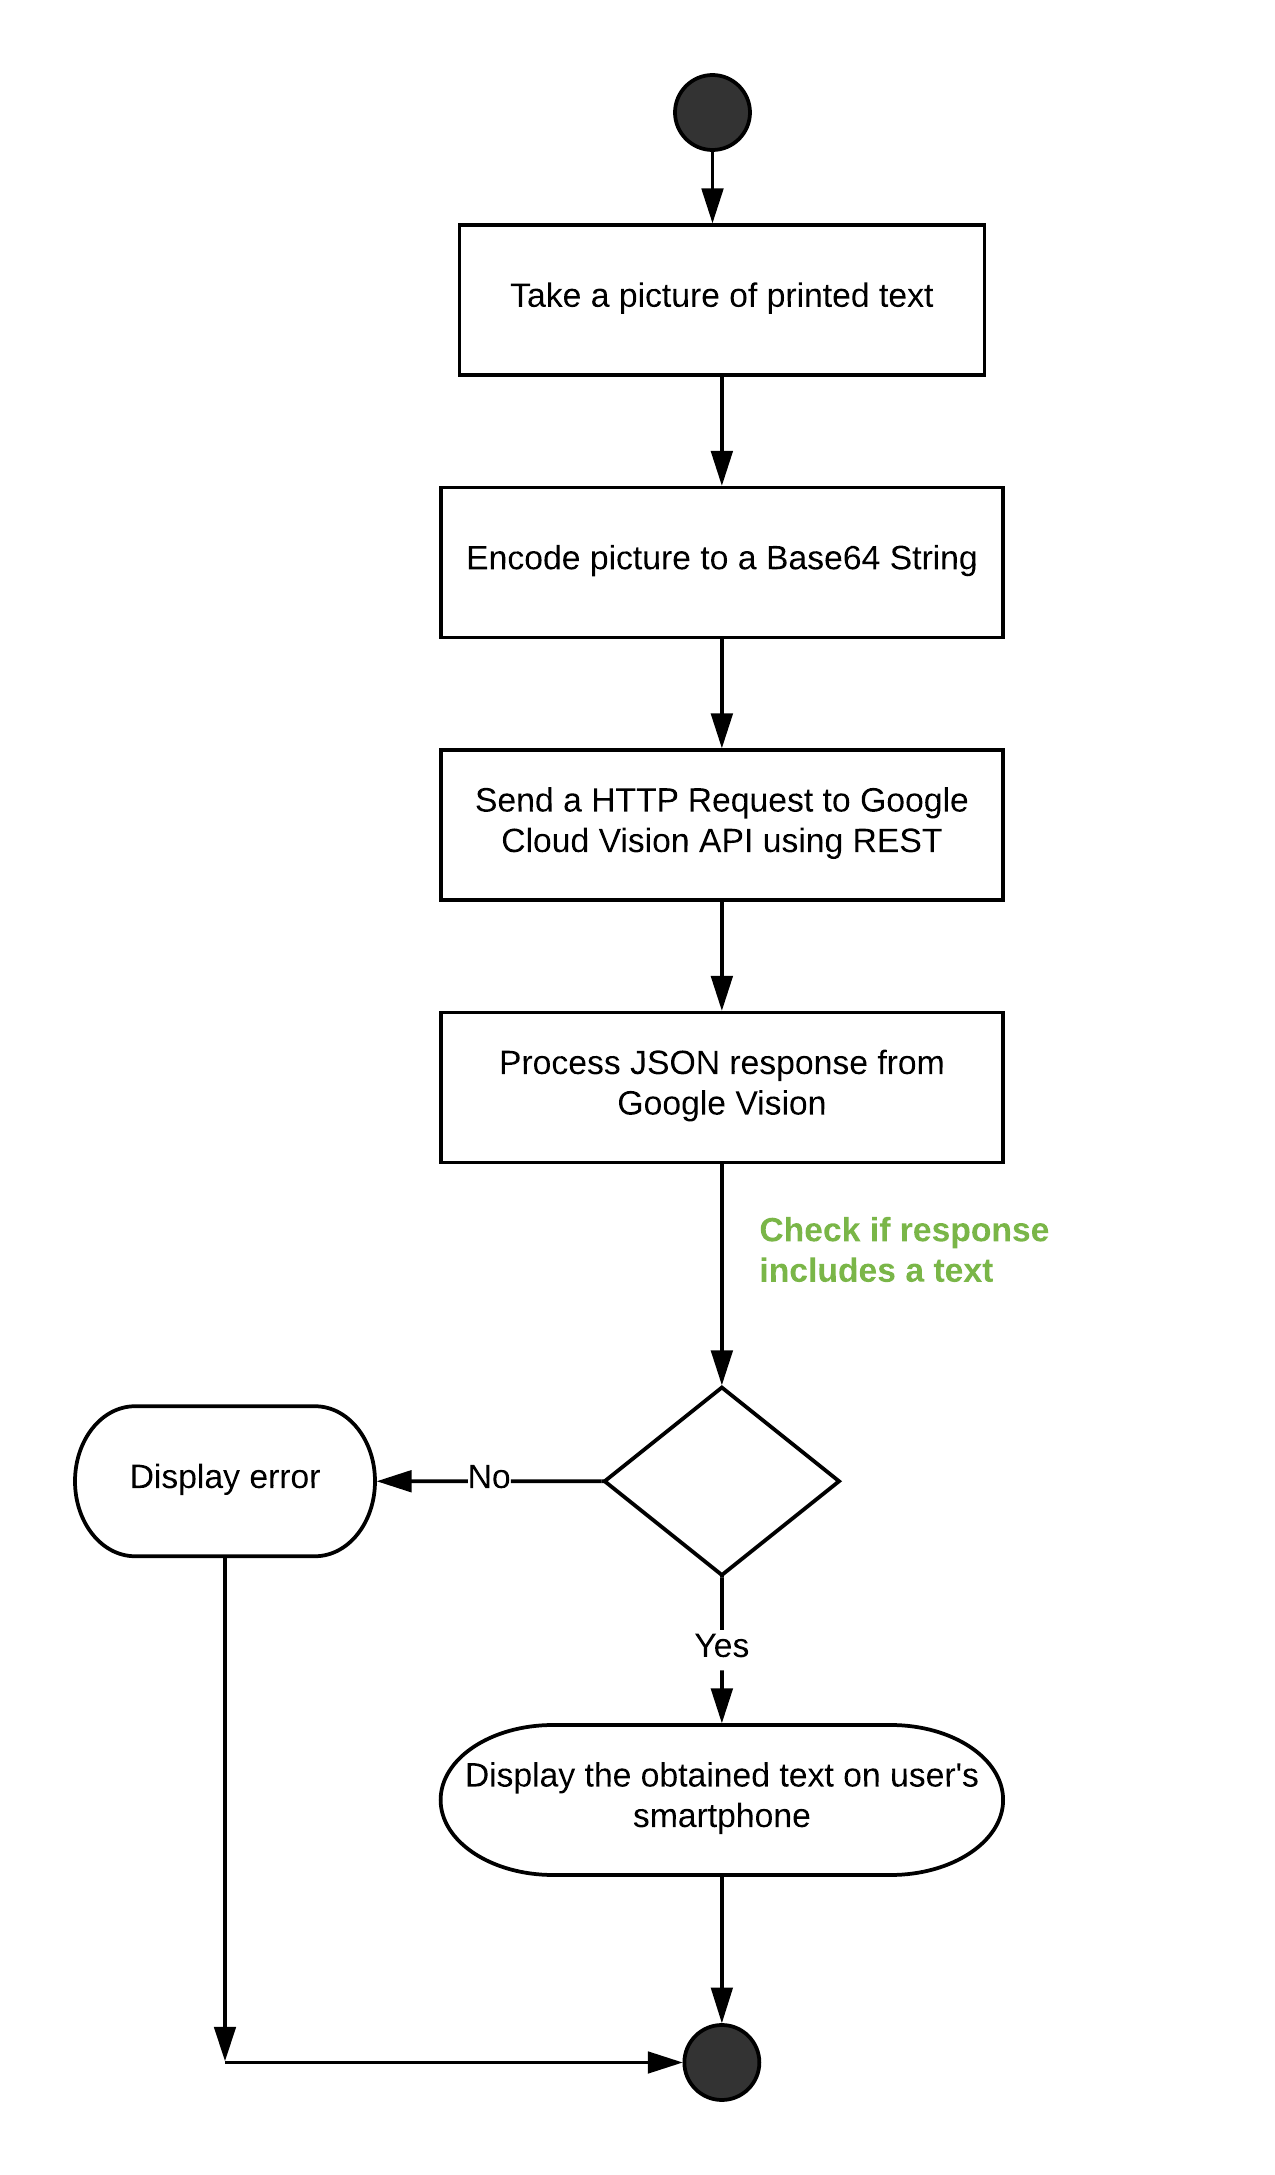
\includegraphics[width=0.75\linewidth]{media/VISION_API.png}
	\caption{UML activity diagram for Text Detection using Google Vision API}
	\label{fig:vision}
\end{figure} 

\subsection{Sample Request}

\paragraph{}Let us consider the image shown in Figure \ref{fig:request_sample} as the source of the image. We use the Algorithm mentioned in Figure \ref{fig:vision} to extract the text from the image.

\begin{figure}[H]
	\centering
	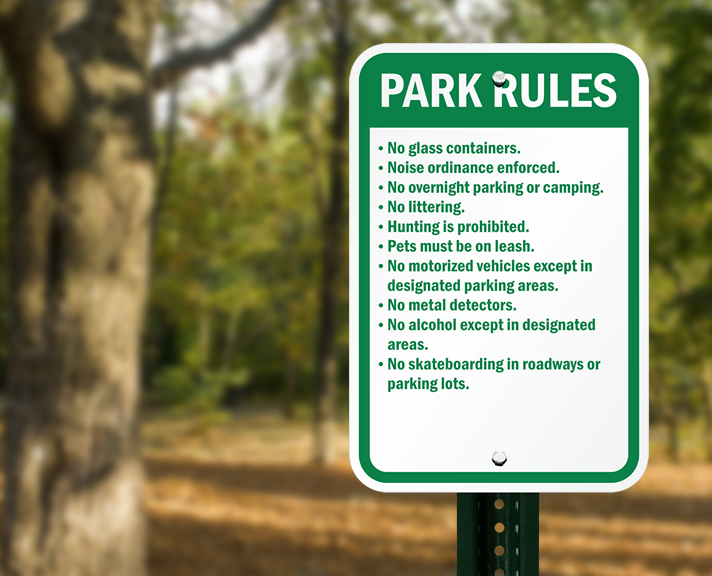
\includegraphics[width=1.0\linewidth]{media/request_sample.png}
	\caption{Example image for testing Google Vision API}
	\label{fig:request_sample}
\end{figure} 

We convert this image to a base64 encoded string using Javascript and specify in the headers of the REST API to use 'Text Detection' feature of Google's Cloud Vision API. A sample request is as shown below:

\begin{lstlisting}
{
	"requests":[{"image":{
	"content":"base64_encoded_string_of_image"
},	
	"features":[{"type":"TEXT_DETECTION",
	"maxResults":1}]}]
}
\end{lstlisting}

\subsection{Sample Response}

\begin{lstlisting}
{
"responses": [{
"textAnnotations": [{
"locale": "en",
"description": "Lorem Ipsum",
"boundingPoly": {
"vertices": [
{"x": 327,"y": 412},{"x": 1158,"y": 412},
{"x": 1158,"y": 680},
{"x": 327,"y": 680}]}}]}]
}
\end{lstlisting}

\paragraph{} In this section, we discussed the capabilities of Google Cloud Vision API and how we implement it into our system. 

\section{Google Cloud Translation API}
\label{translate}

\paragraph{}The Translation API provides a simple programmatic interface for translating an arbitrary string into any supported language using state-of-the-art Neural Machine Translation. It is highly responsive, so websites and applications can integrate with Translation API for fast, dynamic translation of source text from the source language to a target language (such as French to English). Language detection is also available in cases where the source language is unknown. The underlying technology is updated constantly to include improvements from Google research teams, which results in better translations and new languages and language pairs.

\paragraph{}Translation API supports more than one hundred different languages, from Afrikaans to Zulu. Used in combination, this enables translation between thousands of language pairs. Translation API can be accessed using REST APIs. We extract text from the printed signages using Google Cloud Vision API, we then send the text to Google Translate API and convert it into the user's desired language.

\paragraph{}The figure \ref{fig:translate_uml} describes the process of language translation in our system. We obtain the text from the printed media using Google Vision API as mentioned in section \ref{vision}. We then pass the obtained text to Google Cloud Translation API with the preferred language in the headers of REST API. The response from the Google Translate is then displayed in the user's smartphone. A sample request and response is shown below:

\begin{figure}[H]
	\centering
	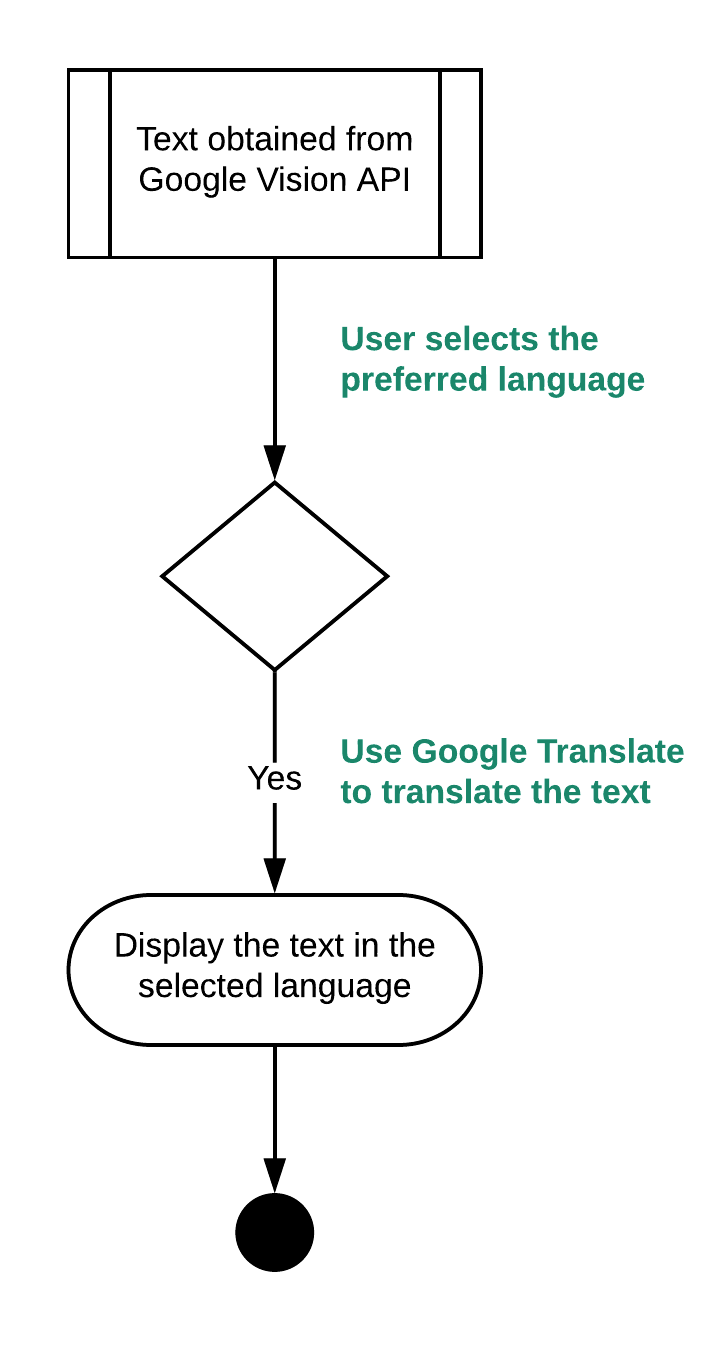
\includegraphics[width=0.5\linewidth]{media/Translate.png}
	\caption{UML activity diagram using Google Translation API}
	\label{fig:translate_uml}
\end{figure} 

\subsection{Sample Request}

\paragraph{}Below code segment shows how to use Google Cloud Translate API using REST APIs using Javascript. Developers should replace their own Google API Key at  API-KEY-HERE. The target language to be translated is passed under 'target' parameter of the REST API. 

\paragraph{}We use javascript to interact with Google Translation API as follows:

\begin{lstlisting}
    fetch(`https://translation.googleapis.com/language/translate/v2
    ?key='API_KEY_HERE', {
      method: 'POST',
      headers: {
        'Accept': 'application/json',
        'Content-Type': 'application/json',
      },
      body: JSON.stringify({
        q: "text_to_be_translated",
        target: "target_language"
      })
    })
    .then(data => data.json())
    .then(res => this.cleanText(res))
    .catch(err => console.log(err))
  }
\end{lstlisting}

\subsection{Sample Response}

\paragraph{} Google processes the requests and responds with a JSON object containing the translated text. A sample response is shown below:

\begin{lstlisting}

{
  "data": {
    "translations": [
      {
        "translatedText": "translated_text_here"
      }
    ]
  }
}
\end{lstlisting}



\section{System Construction}
\label{system}
\paragraph{}In this study, a prototype of multilingual information service system was designed and constructed. 3 beacons was configured and placed next to each of the 3 signage in a park. These beacons continuously broadcast their UUID, major and Minor. A mobile application is developed to listen to these beacons. The mobile application leverages the smartphone’s bluetooth technology to listen to the beacons.

\paragraph{}The relevant information of the signage for each beacon is stored in a database in the cloud. Once the mobile application detects a beacon, it makes a call to the cloud, passing the detected beacon configuration to get the appropriate information of the signage using REST APIs. The information returned from the cloud is then translated to required languages using the Google Translate API and displayed on the user’s smartphone.

\paragraph{}The below figure \ref{fig:system} gives an overview of different processes in our system.

\begin{figure}[H]
	\centering
	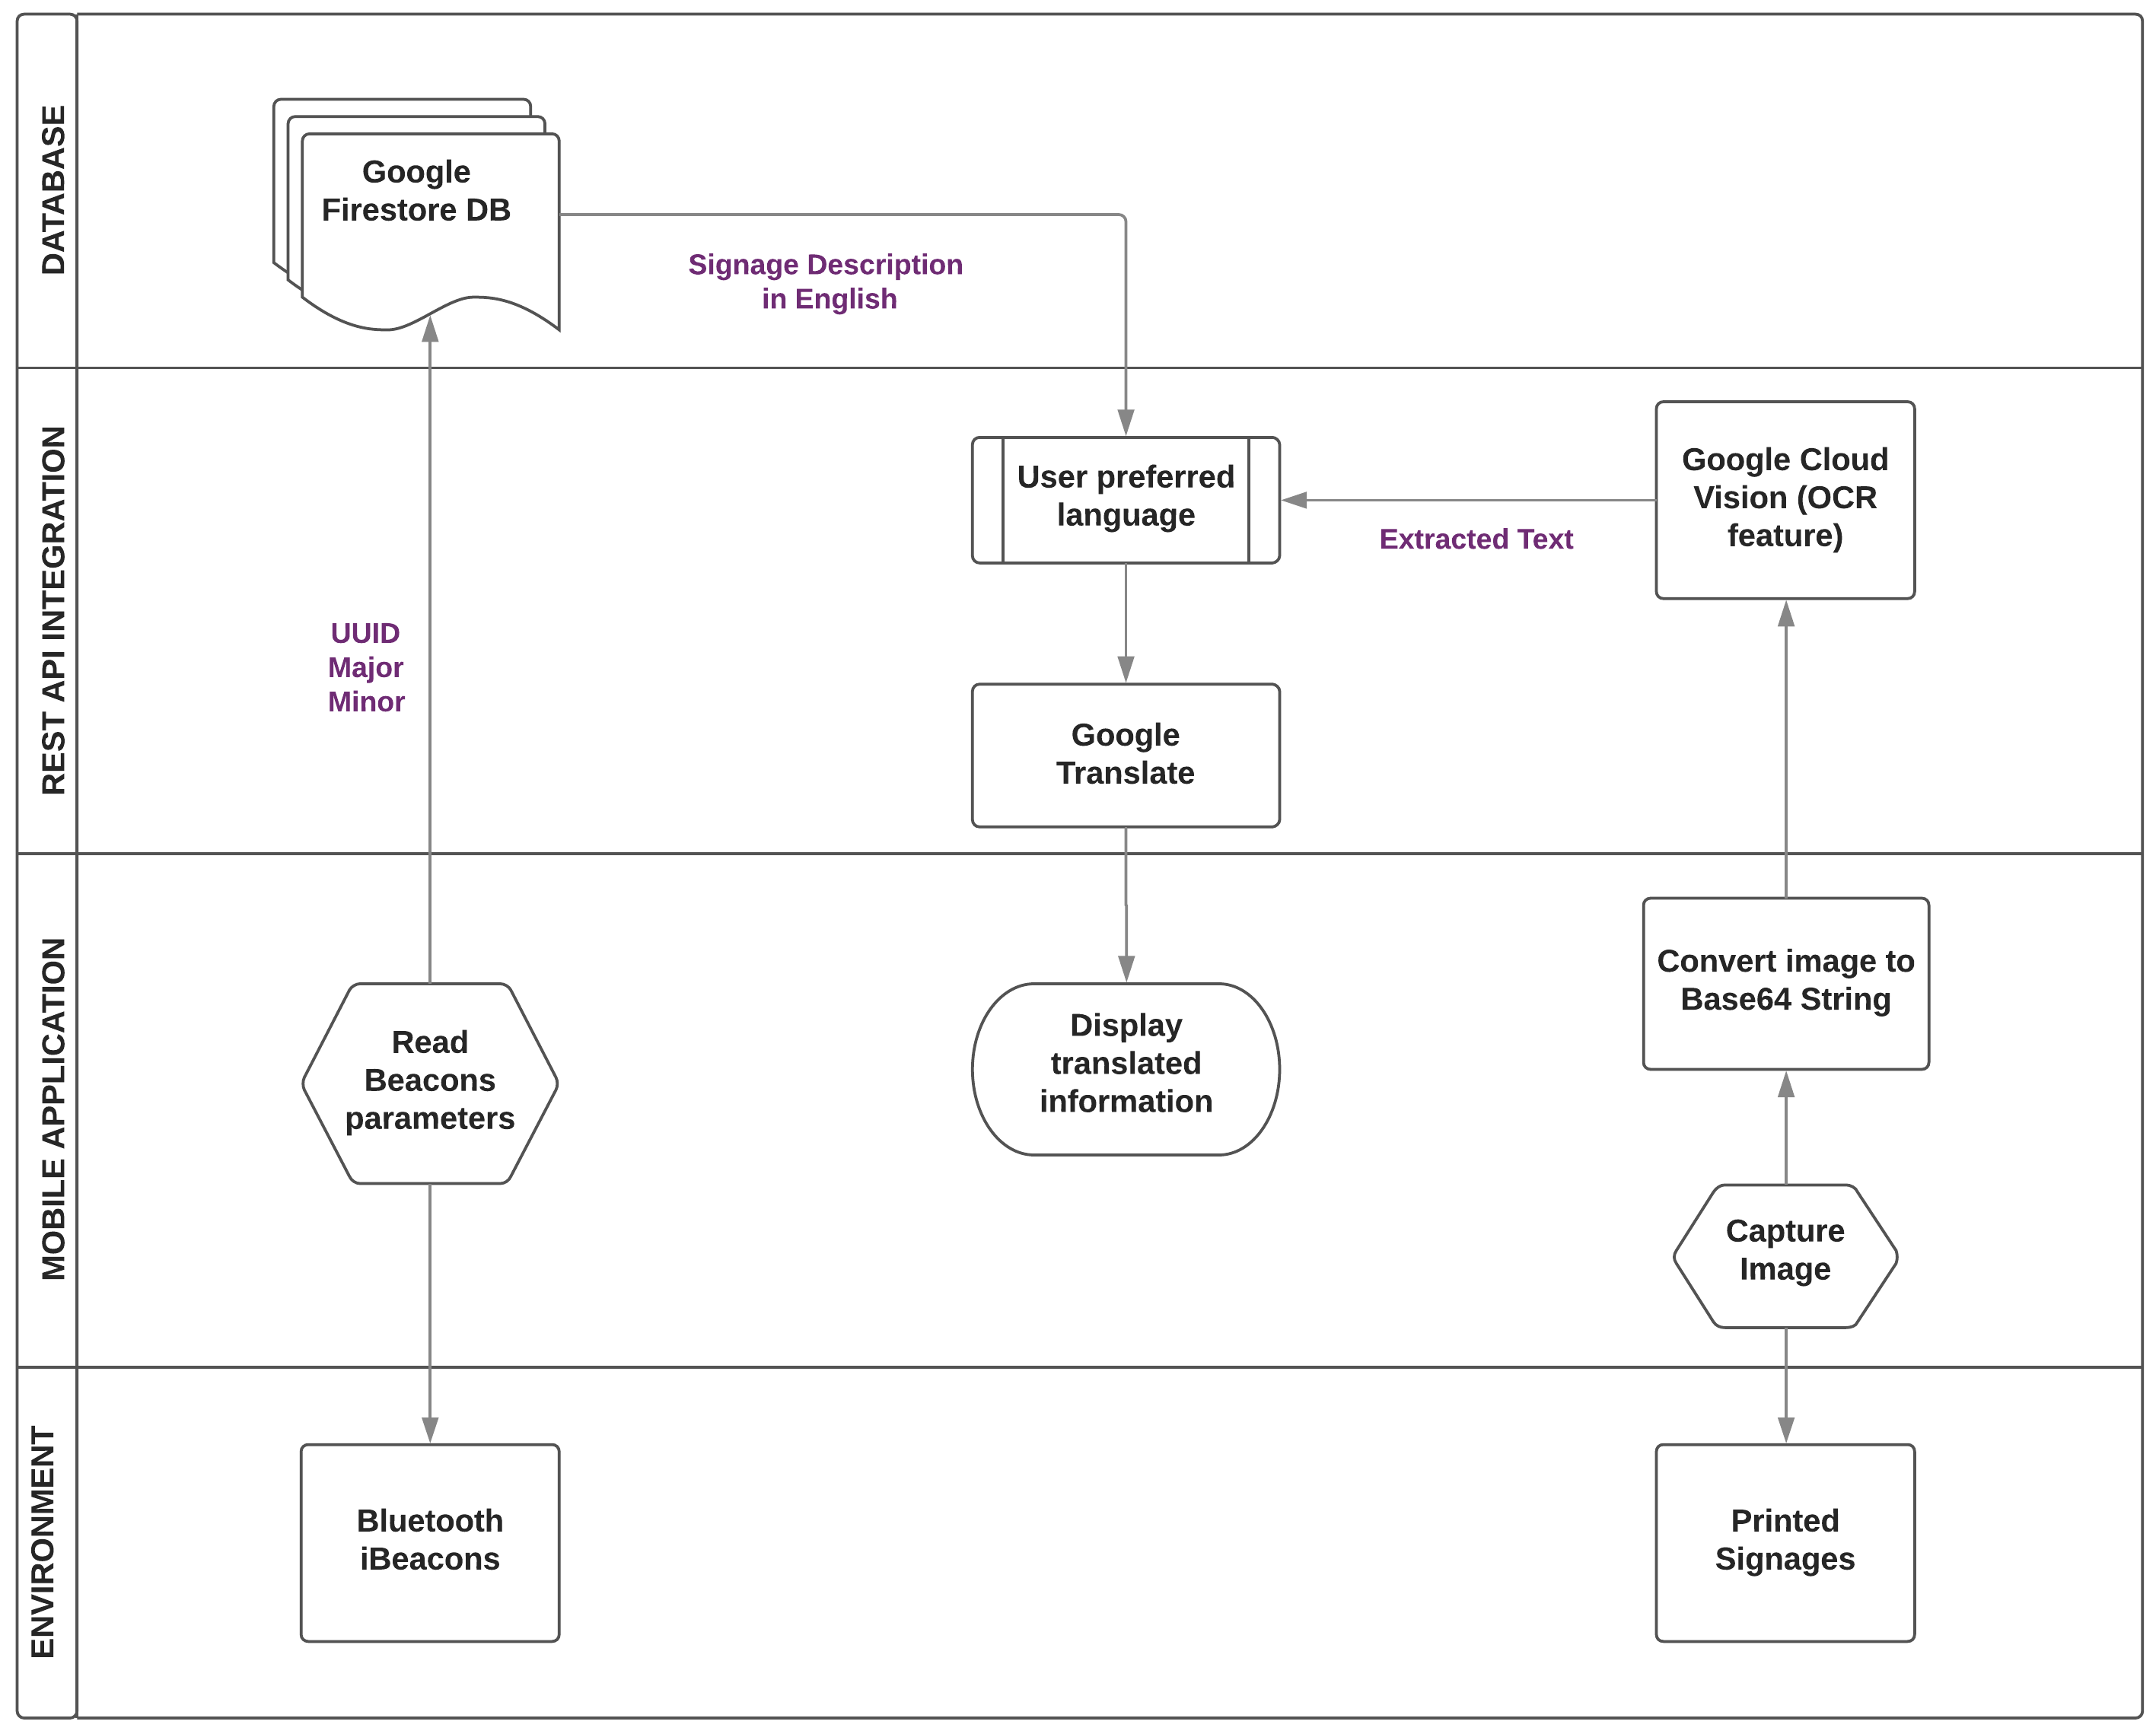
\includegraphics[width=1\linewidth]{media/Architecture-3.png}
	\caption{Process Flow Diagram}
	\label{fig:system}
\end{figure} 

\subsection{Environment}
\label{env}
\paragraph{}To evaluate the system, we constructed a combination of digital signages and printed signages and placed them in the university campus. The students, including foreign students were handed out iPhones running the mobile application and were requested to use our system.

\subsubsection{Digital Signages}
\paragraph{}The digital signage was set up using the Estimote 2018 iBeacons. Each iBeacon is mounted on individual signages in the campus. The beacons are powered by individual CR2032 lithium-ion coin batteries. The users used the iPhone 6s in which the application program that reacts with the iBeacon signals. In this study, we used the iBeacons from www.estimote.com. The parameters of the beacons, which are discussed in the section \ref{iBeacon-tech} can be configured only by the administrator of the mobile application. To evaluate the system, we use 3 beacons. Below are the configurations of each beacons used in the study.

\begin{lstlisting}
UUID: E6FA79C7-804F-4742-863B-BD4D282ED9BA
Major: 1111
Minor: 9991
\end{lstlisting}

\noindent\rule{13cm}{0.4pt}

\begin{lstlisting}
UUID: E6FA79C7-804F-4742-863B-BD4D282ED9BA
Major: 1111
Minor: 9992
\end{lstlisting}

\noindent\rule{13cm}{0.4pt}

\begin{lstlisting}
UUID: E6FA79C7-804F-4742-863B-BD4D282ED9BA
Major: 1111
Minor: 9993
\end{lstlisting}

\subsubsection{Printed Signages}
\label{printed-signages}
\paragraph{}To evaluate our solution of translating the signages without the iBeacons, we printed out commonly used  signages in multiple languages and placed them around the university campus. The students were handed out iPhone 6s, running the same mobile application and were requested to use the system to understand the information on the signages.


\subsection{Mobile application}

\paragraph{}
To discover the beacons from the smartphone, we have designed and developed a mobile application. This mobile application is built using React native and Javascript. The mobile application uses Google Cloud Vision to detect the printed text using the smartphone camera. The Google Cloud Vision API detects the printed information using OCR feature as mentioned in section  \ref{vision}. This text can be converted to any language using Google Cloud Translation API, discussed in section \ref{translate}. The mobile application interacts with these APIs using REST method  To improve the efficiency and user-experience, we used both iBeacon monitoring and ranging to discover and interact with the beacons.


\subsubsection{Background Monitoring}
\paragraph{}Beacon monitoring is similar to geofence, i.e., a virtual barrier that is usually defined using a set of geographic coordinates. In case of iBeacon, the area is defined by the range of one or more beacons. This allows more granularity and precision than regular geofencing. Moving and out of the area it encloses triggers ’enter’ and ’exit’ events, which the app can react to. The smartphone will keep listening for those beacons at all times even if the application is not running in the foreground, and even if the iPhone/iPad is locked or rebooted. Once an ’enter’ or ’exit’ happens, iOS will launch the app into the background (if needed) and let it execute some code for a few seconds to handle the event.

\subsubsection{Beacon Ranging}
\paragraph{} Ranging actively scans for any nearby beacons on the foreground and delivers results to you every second. With monitoring, our app will be notified whenever the user enters and exits the terminal. Ranging for the exact same region, we’ll instead get a full list of matching beacons currently in range - complete with their UUID, major, and minor values.

\subsubsection{Development stack}
\paragraph{} The mobile application was developed after evaluating all the major development tools and technology present in the current market. The main goal is to develop the system, keeping performance and scalability in mind. Also, we want to make sure the system works efficiently on both iOS and Android platforms. Below is the development stack we used to develop the mobile application:

\begin{itemize}
  \item \textbf{React Native:} To develop the front end of the mobile application. The advantage of using React Native is it helps us to develop for both Android and iOS with the same codebase. Also, React Native is efficient in terms of performance.
  
   \item \textbf{JavaScript:} We used Javascript to interact with the web-services such as Google Vision and Google Translate. It makes it efficient to convert the captured images into Base64 encoded string and pass it in the headers of the request. Also, javascript makes it easier to process/parse the JSON response from the web-service and display it on the front-end using React Native. We use Javascript also to communicate with the Google Firestore database to query and retrieve data.
  
      \item \textbf{Camera:} To access the smartphone camera, we included a library called 'react-native-camera'. This extends the functionality of camera in terms of fragments and hence makes it easier to listen to the camera events and implement our logic where necessary.
      
        \item \textbf{Bluetooth:} Our system needs access smartphone's bluetooth module to discover the iBeacons. To check the state of Bluetooth, we included 'react-native-bluetooth-state' library. This helps us determine the bluetooth status of the smartphone, whether 'on' or 'off' and display appropriate messages to the user.
        
        \item \textbf{Beacon Manager:} To discover iBeacons from the smartphone, we integrated 'react-native-beacons-manager' library into React Native. This library helps us scan for the beacons and listen to changes of the beacon signal strength. The library also supports 'background ranging' and 'foreground monitoring' of the beacons, meaning it helps us scan for the beacons even when the application is running in background. 
      
      \item \textbf{Xcode:} To build and run the application on the iOS device, we need an Integrated Development Environment (IDE). Xcode is an IDE that can be used to run the developed mobile application on the iOS device.
      
 \end{itemize}

\subsection{REST API Integration}
\paragraph{} The mobile application developed communicates with the web-services such as Google Cloud Vision and Google Translation using Representational State Transfer (REST).  REST is an 
architectural style that defines a set of constraints to be used for creating web services \cite{rest}. Web services that conform to the REST architectural style, or RESTful web services, provide interoperability between computer systems on the Internet.

\paragraph{}By using a stateless protocol and standard operations, REST systems aim for fast performance, reliability, and the ability to grow, by re-using components that can be managed and updated without affecting the system as a whole, even while it is running. In our system, we interact with Google Vision and Translation web-services through REST method. The response from these web-services is processed in the mobile application and appropriate messages are shown. A sample request and response for each web-services is shown in Sections \ref{vision} and \ref{translate}.

\subsection{Database}
\label{database}
\paragraph{}To store the information of each signage in a database, we chose Google Cloud Firestore. Cloud Firestore is a flexible, scalable database for mobile, web, and server development from Firebase and Google Cloud Platform \cite{firebase}. It keeps the data in sync across client apps through realtime listeners and offers offline support for mobile and web so we can build responsive apps that work regardless of network latency or Internet connectivity \cite{firebase}. Google Firestore is free of cost for less than 50 simultaneous connections to the database, which is a right fit for for the study.

\begin{figure}[H]
	\centering
	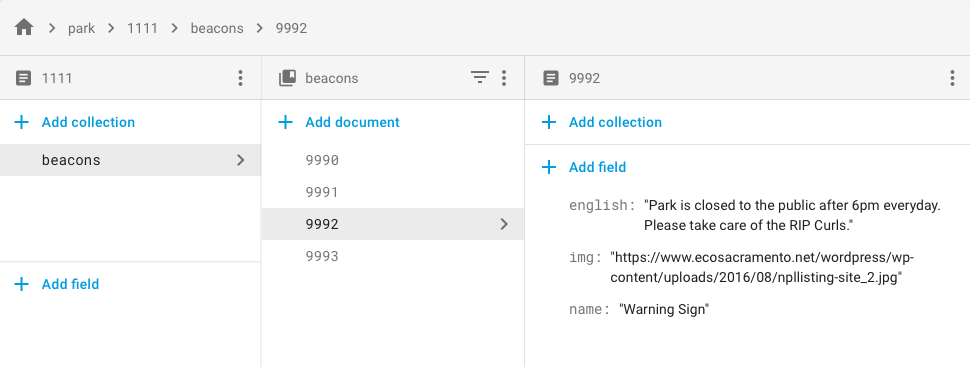
\includegraphics[width=1\linewidth]{media/db.png}
	\caption{Database Schema}
	\label{fig:db}
\end{figure} 

\paragraph{} We designed the database schema with a goal to keep it as simple as possible so it can be scalable in the future. We organize the database schema as follows:

\begin{itemize}
  \item \textbf{Park:} Root of the database. All the beacons with the specified UUID falls under this bucket. 
  
  \item \textbf{1111:} This is the level 1 of the database. This is essentially the 'major' parameter of the iBeacons. Since all the 3 beacons we configured have the same 'major' value, we just have one collection of level 1. This level of database makes it possible for our mobile application to differentiate the sections of the park. This allows the administrator to configure beacon parameters according to sections of the park.
  
  \item \textbf{beacons}: This is the level 2 of the database schema. We now have identified which park the beacons are present in and which section of the park the beacons are present in using the above two levels. 'beacons' section of the database serves as the collection of beacons under a particular section of the park. They contain all the information about the individual beacons present in discovered section.
  
    \item \textbf{9992}: This is the last level of the designed database schema. '9992' refers to the 'minor' value of the iBeacon. Each iBeacon will have its own unique 'minor' value. This helps us to query for the exact beacon data. Each entry at this level have the below fields and values: \\
    
    \textbf{'name':} The name of the signage. \\
    \textbf{'img':} Contains the URL of a picture of the signage. \\
    \textbf{'english' :} This field contains the description of the signage, in English.\\
  
\end{itemize}

\section{Designing the User Experience}
\label{ux}
\paragraph{} Applying UI Design principles and guidelines are very important for developing a mobile-based learning application. By observing user interface design principles and implementing them in the development process, it can be helpful for users to improve usability and grasp critical information as displayed in the application. 

\paragraph{} For this study, set of User Interface Design (UID) principles is considered \cite{uid} for designing and developing the mobile-based multi-lingual signage application. Below are the set of UIDs adopted:

\begin{itemize}

 \item  Navigation should be simple and clear from a page to
any particular section. In short, the navigation should be
consistent throughout all pages in an application.

 \item  Complex navigation needs to be avoided by the
developer on the application.

 \item Reduce scrolling frequently.

 \item Application should be user-friendly and allow
users to understand how the application works intuitively.

 \item Similar actions and information need to be located in
similar positions. For instance, similar buttons must be
found in similar positions for the whole pages of the
application.

 \item Flexibility of the display is the significant property for
usability of interface design.

 \item Providing necessary information only. Unnecessary
information confuses the learners and decreases their
performance.

 \item  Decreasing textual information and increasing
information which is provided in graphical media to minimize learners' cognitive load and motivate
them to keep using the application.

\end{itemize}


From the psychological point of view, interface design can be divided into feeling (visual, auditory and tactile etc) and emotional levels. User interface design is an important part of on-screen aplications. Interface design is a complex engineering which have different disciplines in, cognitive psychology, design, linguistics, etc. \cite{hci}. There are three main principles of User interface design:  Intuitive user interface, Reduce the burden of user memory, maintain the consistency of the interface. 


\paragraph{}We are going to carefully design the User Interface (UI) and User Experience (UX) based on the best practices for Human Computer Interaction (HCI). Below sections describe the concepts behind designing the UI and UX.

\subsection{User Analysis}

Below are the different types of users we expect to use our system:

\begin{itemize}

 \item \textbf{Primary Users:} People who visit foreign countries either for tourism or business. Usually, the signages are displayed in local languages. This is a hindrance to visitors. They would want to understand their surroundings.
 
  \item \textbf{Secondary Users:} Visitors of parks and exhibits who would like to know more about their surroundings in their native language. The application will scan for digital signages and present relevant information once the user is in proximity.
  
  \item \textbf{Tertiary Users: } Tertiary users are the users who interact with the translated information. They may be the native people interacting with the visitors. 
  
\end{itemize}

\subsubsection{Example Persona}
\label{persona}

This section describes an example persona of a primary user:

\paragraph{}Rebecca is a freshman in the Environmental Sciences program. She is 22 years old,
from Arlington, VA. Throughout her high school years, she has been interested in preserving the environment, and has been involved in numerous recycling and conservation activities. She has had various international travel experiences, including a trip to Japan for a youth group ministry project.

\paragraph{} Rebecca lives on campus in the dorm she shares with two other college students. She is very comfortable with technology and uses Twitter, Facebook, and email to communicate with friends and family. Rebecca believes in technology to reach out to people and spread knowledge about
Amazon rainforests through images and icons. Rebecca is motivated to participate in a Peruvian conservation project during the summer following her high school graduation. She is the current Vice President of the Environmental Society.

\paragraph{} During her foreign travels with the society, especially to the national parks, Rebecca likes to understand more about the environment and always makes sure there is enough signages so people are aware of the rules and do not pollute the environment. 

\subsection{Task Analysis}
\label{task}
\paragraph{}In this section, we identify what the user is trying to achieve using our system. We also identify the tasks that need to be supported in order for the user to achieve his goal. Below are the list of tasks the system needs to support. 

\begin{itemize}

 \item The system needs to support taking pictures of the signage and extract the printed text. 
 
  \item The system needs to translate text into the user's preferred language.
 
  \item The application should remember the selected language and display the translated text into the preferred language.
  
  \item The application should scan for digital signages and display the distance of the user from the signage.
  
    \item The application should fetch the appropriate information from the database and display the same.
    
    \item The administrator of the system should be able to configure the beacons and change the fields of the database as well.
    
    \end{itemize}
    
    \subsection{Context Analysis}
    
    In this section, we discuss where the developed system can be used. We also discuss the social and environmental conditions. Below are the environments our system could be used:
    
   
\begin{itemize}

 \item In parks and exhibits that involve multiple signages.
 
  \item Museums, where there is a need for foreign visitors to understand the signages in their native language.
 
  \item In shopping malls, so visitors can understand critical information and navigate easily.
  
  \end{itemize}
  
    \subsection{Design Principles}
    
    The user experience was designed according to the design principles of Human Computer Interaction (HCI). In this section, we discuss the various design principles incorporated in designing the UX. 
    
    \subsubsection{Affordance}
    \paragraph{}According to Donal Norman (1988) an affordance is the design aspect of an object which suggest how the object should be used; a visual clue to its function and use \cite{norman}. Affordance is a property in which the physical characteristics of an object influence its function. 
    
    \paragraph{} In the mobile application developed, the UI of the Landing page (shown on opening the application) is divided into 2 sections. About 3/4th of the screen shows the camera view, which means the application is ready to capture a picture of printed signages and extract text from it using Google Cloud Vision. The rest of the screen shows the nearby digital signages. The application also shows the distance between the digital signage and the user.
    
     \subsubsection{Visibility}
     \paragraph{}The usability is improved when its status and methods of use are clearly visible. The more visible functions are, the more likely users will be able to know what to do next.\cite{norman} In contrast, when functions are 'out of sight,' it makes them more difficult to find and know how to use.
     
         \paragraph{} In the mobile application developed, the capture picture button has a green color, so as to invite the user to click the button. The camera functionality also has an 'upload image' icon and 'type and translate' icon present upfront. Their is no ambiguity in the user interface. The digital signage section also lists the nearby digital signages along with the title and distance from the user. This improves the visibility of all the features of the app without the user having to scroll down. 
     
      \subsubsection{Constraint} 
      
      \paragraph{}The design concept of constraining refers to determining ways of restricting the kind of user interaction that can take place at a given moment \cite{norman}. This helps the application to do what it is exactly supposed to do and eliminates many error scenarios. This is helpful for the stable functioning of the application.
      
      \paragraph{}In the system we built, we establish constraints by only listing the digital signages around. If there are no digital signages around, 'No digital signages around' message is shown to the user. Also, the system is constrained to capture/upload only one image and use web-services to extract text from it. This helps the application function without many errors. 
      
      
      
       \subsubsection{Consistency}
       \paragraph{}This refers to designing interfaces to have similar operations and use similar elements for achieving similar tasks \cite{norman}. In particular, a consistent interface is one that follows rules, such as using the same operation to select all objects. This helps the user intuitively learn and use the application without having to spend more time on it \cite{norman}. 
       
       \paragraph{}In our study, we have designed the UI using the modules approach. That is, whether the user chooses to capture an image or upload from the camera roll, the layout is the same. In the digital signages section, all the signages are listed consistently and the whole thumbnail is clickable. Each click takes the user to a screen with more details about the signage. This page is designed consistently. This helps the user to understand our application faster.
       
        \subsubsection{Feedback}
       \paragraph{}Feedback is about sending back information about what action has been done and what has been accomplished, allowing the person to continue with the activity \cite{norman}. This helps the user to understand there is a background process running and at the same time, the user is constrained from starting another process or quitting the current process. 
       
       \paragraph{}In the application developed, the user is shown 'loading' icon when a background process is running, for example, when an image is being uploaded through web-services. This helps the user understand that there is a process running in the background and also helps the user to understand the application better. Also, appropriate error messages are shown at the appropriate places to help user understand about the action being carried out \cite{norman}.
       
    
    



\section{Conclusion and future work}
\label{sect-conclusion}
Your work goes here

\cleardoublepage
\phantomsection
\bibliographystyle{plain}
\bibliography{references}
\addcontentsline{toc}{section}{References}

\end{document}

